\documentclass{standalone}

\usepackage{tikz}

\begin{document}
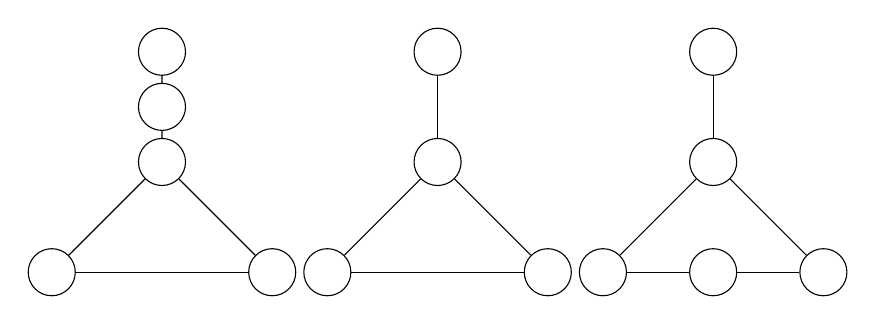
\begin{tikzpicture}[scale=.7]
\tikzstyle{vertex}=[circle, draw, minimum size=17pt, inner sep=0pt]
\node[vertex] (A) at (0,0) {};
\node[vertex] (B) at (4,0) {};
\node[vertex] (C) at (2,2) {};
\node[vertex] (D) at (2,3) {};
\node[vertex] (E) at (2,4) {};

\path 
(C) edge (A)
    edge (B)
    edge (D)
(D) edge (E)
(A) edge (B);

\begin{scope}[xshift=5cm]
\node[vertex] (G) at (0,0) {};
\node[vertex] (H) at (4,0) {};
\node[vertex] (I) at (2,2) {};
\node[vertex] (J) at (2,4) {};

\path 
(I) edge (G)
    edge (H)
    edge (J)
(G) edge (H);

\end{scope}


\begin{scope}[xshift=10cm]
\node[vertex] (Z) at (0,0) {};
\node[vertex] (Y) at (4,0) {};
\node[vertex] (X) at (2,2) {};
\node[vertex] (W) at (2,4) {};
\node[vertex] (V) at (2,0) {};

\path 
(X) edge (Z)
    edge (Y)
    edge (W)
(V) edge (Z)
    edge (Y);

\end{scope}

\end{tikzpicture}




\end{document}
